\documentclass[10pt]{article}
\usepackage[margin=0.68in]{geometry}
\usepackage[T1]{fontenc}
\usepackage{lmodern}
\usepackage{microtype}
\usepackage{booktabs}
\usepackage{longtable}
\usepackage{amsmath}
\usepackage{array}
\usepackage{graphicx}
\usepackage{float}
\usepackage[hidelinks]{hyperref}
\newcommand{\artifact}[2]{\href{#1}{\texttt{#2}}}
\newcommand{\sha}[1]{\par\noindent{\small\texttt{#1}}\par}
\title{Supplement S3: External protocol and budget results to ``What Does a Persona Add?''\\
\large Evidence lineage, paired capacity comparison, and external stimulus protocol}
\author{Anonymous authors}
\date{}
\begin{document}
\maketitle

\section{Scope and source lineage}
This supplement records the retrospective B1 capacity comparison and R2 stimulus-matched protocol and results. The historical diagnostics are supplied separately as Supplement S4. Protocol freezing is internal, not public preregistration.

The external source is \texttt{LLM-Digital-Twin/Twin-2K-500}. Its pinned
revision is
\sha{f883165a3026fde855dfd448e0cd16443ab257b6}
The original
49-endpoint catalog protocol is
\texttt{TWIN\_PROTOCOL\_FROZEN.json}.
Its file SHA-256 is
\sha{0ea4652877ccc93b288e71172fb5a4d473985c431b794fb095434746622fae17}
The respondent-specific R2 amendment is
\texttt{TWIN\_STIMULUS\_AMENDMENT.json}.
Its SHA-256 is
\sha{1a968951bbf7f11a5d9a838b00676e058de1896a7778bece04ba0b1d3eb70067}
It binds the parent protocol, prepared receipt, question-only sidecar, FIT
orientation audit, canonical target-count ledger, and presentation-slot
response semantics. The source and FIT-only receipts are the
\texttt{source audit}
and \texttt{FIT orientation audit}. The R2 amendment
was frozen \emph{after} the earlier v6 history-only CAL readback but
\emph{before} any R2 fit or GPU forecast. All 84 compute cluster source tests and
complete R2 input validation are engineering checks, not predictive results.

\section{B1: complete paired capacity comparison}
\label{sec:b1}
The target is normalized ordinal ranked probability score (RPS) on 60
disjoint target items for each of the same 600 E3 people. For $K$ categories,
\[
 \operatorname{RPS}(p,y)=\frac{1}{K-1}\sum_{k=1}^{K-1}
 \left(\sum_{j=1}^{k}p_j-\mathbf{1}\{y\leq k\}\right)^2.
\]
Lower is better. The contrast is the archived E3 frozen hybrid minus the
within-budget, cross-validated statistical predictor. The hybrid's
per-person loss is averaged across nine fixed correlated combinations
(three old LLM seeds times three ridge subset seeds); the reference's
per-person loss is averaged across three fixed subset seeds. Forecast
probabilities are scored before averaging losses. The nine historical
combinations are not nine independent optimizer runs. The 600 respondent
differences, not individual item answers, are the inferential units.

At each budget $n\in\{80,160,320,1000,8000,8320\}$ and in each of the
raw-answer and exact categorical-profile representations, the frozen
candidate families were an empirical prior, ridge penalties
$\{1,10,100,1000\}$, and a small nonlinear kNN/ExtraTrees family. Within
each $n$ and each of three nested subset seeds, three-fold training-only
cross-validation selected family and hyperparameters by mean held-person
RPS, with registered ties. The $8,320$ pool comprises the historical
Train8000, Search80, Select120 and Calibrate120 people; no E3 Eval600 label
entered fitting or selection. All 18 budget-by-seed selections and 108
family forecasts were retained. The historical hybrid itself nevertheless
used additional search, prior, selection and calibration supervision, so
$n$ is a \emph{statistical fit budget}, not total unique human information
or literal questionnaire answers saved.

\begin{longtable}{@{}rllrr@{}}
\caption{All 12 retained B1 contrasts. $\Delta$ is hybrid minus selected
reference normalized RPS; positive favors the reference. Intervals resample
600 respondents conditional on fixed forecasts. $p_{H,12}$ is the separate
12-contrast secondary Holm family; the two $n=8320$ rows have primary
Holm-adjusted $p_{H,2}=0.0004$.}\label{tab:b1}\\
\toprule
$n$ & History & $\Delta$ & Conditional 95\% CI & $p_{H,12}$\\
\midrule\endfirsthead
\toprule $n$ & History & $\Delta$ & Conditional 95\% CI & $p_{H,12}$\\
\midrule\endhead
80   & Raw         & $-0.007086$ & $[-0.007705,-0.006471]$ & 0.0024\\
160  & Raw         & $-0.000500$ & $[-0.001047,\phantom{-}0.000066]$ & 0.0820\\
320  & Raw         & $\phantom{-}0.005355$ & $[0.004644,0.006076]$ & 0.0024\\
1000 & Raw         & $\phantom{-}0.012844$ & $[0.011920,0.013785]$ & 0.0024\\
8000 & Raw         & $\phantom{-}0.021580$ & $[0.020406,0.022741]$ & 0.0024\\
8320 & Raw         & $\phantom{-}0.021679$ & $[0.020556,0.022857]$ & 0.0024\\
80   & Categorical & $-0.008770$ & $[-0.009444,-0.008102]$ & 0.0024\\
160  & Categorical & $-0.002250$ & $[-0.002824,-0.001697]$ & 0.0024\\
320  & Categorical & $\phantom{-}0.004270$ & $[0.003631,0.004925]$ & 0.0024\\
1000 & Categorical & $\phantom{-}0.011452$ & $[0.010559,0.012307]$ & 0.0024\\
8000 & Categorical & $\phantom{-}0.018254$ & $[0.017158,0.019373]$ & 0.0024\\
8320 & Categorical & $\phantom{-}0.018311$ & $[0.017188,0.019426]$ & 0.0024\\
\bottomrule
\end{longtable}

The receipt records 5,000 respondent bootstrap draws and 5,000 paired
two-sided sign flips. Both $n=8320$ primary contrasts have Holm-adjusted
$p=0.0004$, but neither passes the \emph{benefit} gate: $\Delta\leq-0.001$,
upper CI below $-0.001$, and Holm $p<0.05$ were all required together.
At $n=80$ the hybrid leads despite its hidden historical supervision;
$n=160$ differs by representation; from $n=320$ both selected references
lead. These are conditional estimates on the already exposed E3 panel.

\section{R2 respondent-specific stimulus crosswalk}
\label{sec:crosswalk}
The original catalog stores the first question it saw for a QID, while the
survey presented 40 product categories in randomized slots and with
respondent-specific prices. A question-only source scan read the respondent
ID and source question objects, not the Wave-4 numeric answer column. For
each respondent it masked exactly one posted price, matched the remaining
text to a canonical product, preserved that product's actual price and
ordered options, and checked that every product appeared once. The nine
nonpricing target texts and options were invariant. The full ledger is:

\begin{center}
\begin{tabular}{@{}lr@{}}\toprule
Verified item & Count\\\midrule
Respondents / canonical endpoints & 2,058 / 49\\
Product offers / products per respondent & 82,320 / 40\\
Product-slot pairs observed & 1,600\\
Price levels per product / zero-price offers & 11 / 7,490\\
Offers exactly matching old catalog example & 220\\
Nonpricing endpoints with invariant text/options & 9\\
FIT-only question-text matches & 43,000 / 43,000\\
FIT-only numeric slot-choice agreements & 49,000 / 49,000\\
\bottomrule\end{tabular}
\end{center}

\begin{figure}[H]
\centering
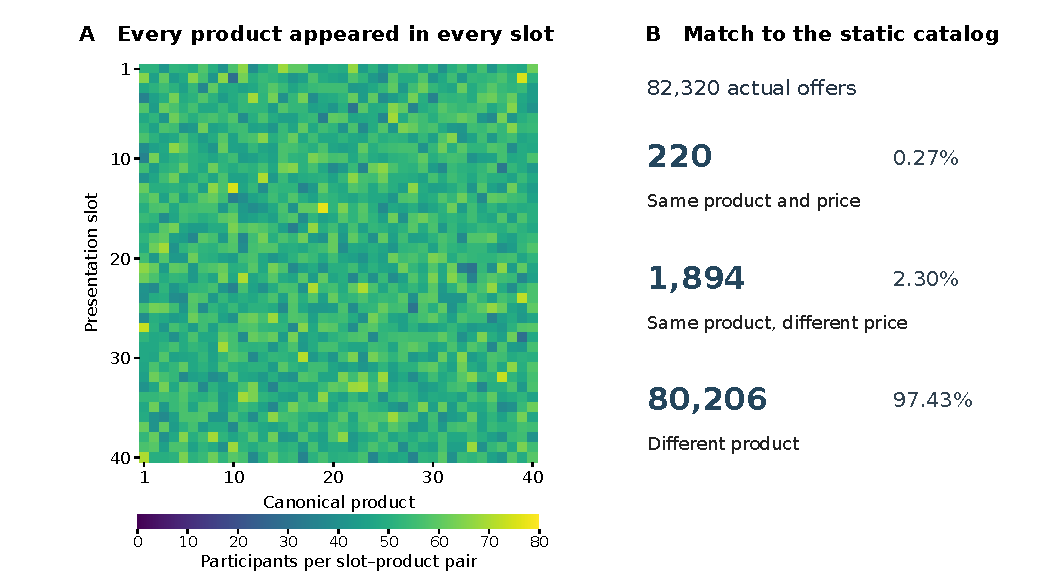
\includegraphics[width=0.82\linewidth]{stimulus-alignment.pdf}
\caption{Outcome-blind product-by-presentation-slot counts (left) and
comparison with the static catalog example (right). Of 82,320 actual
offers, 220 matched both catalog product and price, 1,894 matched product
but not price, and 80,206 displayed a different product in the catalog's
slot. Counts derive from question text and price only; no participant
answer enters the figure.}
\label{fig:alignment}
\end{figure}

The numeric orientation audit inspected only the 1,000 frozen FIT people to
establish that \texttt{QID9\_j} numeric response columns index randomized
\emph{presentation slots}. Its 49,000 agreements connect selected option
positions in the source question object to the numeric export. DEV, CAL and
TEST answers were not inspected for this orientation check; no predictive
model was fit or scored by it. R2 maps a raw slot answer to a canonical
product answer using the verified question-only slot/product permutation.
Both LLM arms receive the exact respondent question and both statistical
controls receive the same product/price/condition fields. The sidecar,
amendment, option order, counts and source code are hash-bound at input
load and comparison. The earlier v6 history-only CAL result (prior chosen
for 45 of 49 endpoints) marginalizes over this offer variation and does
not measure whether history adds value conditional on a known offer.

\section{External endpoints, scoring, and primary aggregation}
\label{sec:external}
The frozen endpoint definition is in
\texttt{TWIN\_PROTOCOL\_FROZEN.json}; the following table fixes
its groups and scales without disclosing participant data.

\begin{center}
\begin{tabular}{@{}p{0.23\linewidth}p{0.33\linewidth}cp{0.22\linewidth}@{}}\toprule
Family & Canonical columns & $K$ & Primary score\\\midrule
Economic preferences & \texttt{QID9\_1--QID9\_40}, 40 canonical products & 2 & Exact log loss\\
Heuristics/cognitive bias & \texttt{QID288\_1--4}, \texttt{QID289\_1--4}, eight ratings & 7 & Normalized RPS\\
Heuristics/cognitive bias & \texttt{QID196}, one binary choice & 2 & Exact log loss\\
\bottomrule\end{tabular}
\end{center}

All probabilities must match every respondent, endpoint, ordered option and
split. Missing human labels use one fixed observed mask per endpoint across
all methods; missing \emph{forecasts} fail the panel. For nominal/binary
endpoints, $L(p,y)=-\log p_y$ without clipping; $p_y=0$ yields infinite loss
and unavailable aggregate inference. Brier is secondary. For the eight
ordinal tasks, $L$ is the normalized RPS above with $K=7$.

The frozen primary overall estimand is dimensionless. Let $D_e$ be the
mean CAL primary loss of the FIT1000-only Laplace prior with $\alpha=1$
for endpoint $e$ (zero history). For a system $S$ and reference $R$, let
\[
 \delta_e=\frac{1}{|O_e|}\sum_{i\in O_e}
 \frac{L_{ie}(S)-L_{ie}(R)}{D_e},\qquad
 \Delta=\frac12\left(\frac1{40}\sum_{e\in E_{40}}\delta_e\right)
       +\frac12\left(\frac1{9}\sum_{e\in H_9}\delta_e\right).
\]
Here $O_e$ is the fixed set of observed TEST labels at endpoint $e$.
The freeze records each prior vector, FIT and CAL labeled counts, and
$D_e$; $D_e\leq10^{-6}$ or no CAL labels aborts. Every endpoint needs at
least 30 observed TEST labels or the \emph{entire} primary aggregate is
unavailable. This averages normalized \emph{differences} within endpoint,
then endpoints within family, then the two families equally; it never pools
raw log loss and RPS. The three-subfamily variant was explicitly not chosen
as primary. A respondent bootstrap or sign vector is shared across all 49
endpoints, retaining within-person dependence. Empty-mask bootstrap draws
are counted and the valid-draw conditional CI and failure fraction reported.
Holm correction covers the complete 12 primary system-versus-full1400
contrasts separately from the two T0-versus-neutral contrasts; endpoint
tables use a separate secondary Holm family.

\section{Frozen model, comparator, and failure gates}
\label{sec:gates}
The R2 statistical family includes an empirical Laplace prior and
predeclared regularized logistic and ExtraTrees candidates using history,
respondent-specific stimulus, or both. Three-fold CV inside the 1,200
FIT+DEV people is specified to choose each endpoint's family and settings
before CAL or TEST scoring. The \texttt{decoder1200} CAL forecast must be
held out. The \texttt{full1400} comparator is specified to refit using
FIT+DEV+CAL and to be scored only on TEST; its in-sample CAL output is
ineligible for mixture tuning.

The two fixed LLM arms are neutral and the portable T0 instruction
component, on each pinned model. The instruction is not the full old NEO
genotype. A CPU preflight binds source hashes, model/tokenizer commits,
architecture, exact complete prompt tokenization and a no-truncation context
ceiling. A finite one-GPU DEV probe tests 10 people across every endpoint
and both arms before CAL. Each forecast is the exact full-softmax mass on
registered canonical digit tokens, normalized within that set; the frozen
minimum digit-mass gate must pass. CAL alone is designated to choose, per arm and endpoint,
$w\in\{0,0.1,\ldots,1\}$ for $wP_{\rm LLM}+(1-w)P_{1200}$ by the endpoint's
primary score. The fixed $w=0.5$ mixture is also retained. TEST starts only
after the mixture freeze binds the R2 stimulus lineage, prepared source,
options, and same model/readout. Direct arms, fixed mixtures and selected
mixtures are all compared to full1400 without outcome-based deletion.

An incomplete forecast grid, mismatched labels or options,
source-hash drift, failed digit-mass/context gate, nonfinite probability or
unbound receipt is a failed or unavailable comparison, never an imputed
zero effect. Exact-zero true-answer log loss remains infinite; no clipping
or selective method dropout repairs it. Scores retain negative, mixed and
failed rows. One model's engineering failure does not certify a scientific
effect for the other. TEST remains sealed until the declared gates pass.

\section{Resource and exposure ledger}
\label{sec:cost}
Finite Slurm allocations are required for CPU prepare/selection/scoring and
for single-GPU model inference. Receipts distinguish allocated CPU-hours,
allocated GPU-hours, elapsed seconds, prompt tokens, attempted/completed
forecasts, failed tasks, and unknown fields; an absent field is \emph{unknown},
not zero. Both DEV models produced 980 forecasts; their combined GPU
allocation was 1.69 hours. The pilot-based resource forecast for CAL and
TEST was 218.52 GPU-hours across both models. The two CAL and two TEST GPU allocations used 143.89 hours in total. The historical minimum of 300.60
allocated GPU-hours excludes known-unsummed search/development and failure
components, so it is not an end-to-end cost ratio against the fitted
statistical controls. The external Wave-4 labels are public, model
pretraining exposure is unknown, and the instrument measures hypothetical
answers rather than purchases.

AI assistance is disclosed in the main manuscript.

\section{Verified external TEST results}
\noindent The separate numerical audit reconstructed all 14 primary and 686 endpoint contrasts, including the frozen respondent bootstrap and sign-flip draws. Negative values favor the system. The two contrasts against neutral form their own Holm family.
\begin{center}\small\begin{tabular}{llrrr}\toprule System & Reference & $\Delta$ & 95\% interval & Holm $p$\\ \midrule
Granite Neutral & Full1400 & 0.43267 & [0.41554, 0.44938] & 0.0024\\
Granite Neutral half & Full1400 & 0.09614 & [0.08774, 0.10418] & 0.0024\\
Granite Neutral CAL & Full1400 & -0.00404 & [-0.00723, -0.00096] & 0.0360\\
Granite T0 & Full1400 & 0.37564 & [0.35879, 0.39205] & 0.0024\\
Granite T0 half & Full1400 & 0.08115 & [0.07308, 0.08924] & 0.0024\\
Granite T0 CAL & Full1400 & -0.00384 & [-0.00692, -0.00085] & 0.0486\\
Granite T0 & Granite neutral & -0.05703 & [-0.06204, -0.05193] & 0.0004\\
Qwen Neutral & Full1400 & 0.30872 & [0.29367, 0.32358] & 0.0024\\
Qwen Neutral half & Full1400 & 0.06902 & [0.06117, 0.07686] & 0.0024\\
Qwen Neutral CAL & Full1400 & -0.00202 & [-0.00503, 0.00106] & 0.4107\\
Qwen T0 & Full1400 & 0.33939 & [0.32222, 0.35712] & 0.0024\\
Qwen T0 half & Full1400 & 0.07664 & [0.06800, 0.08536] & 0.0024\\
Qwen T0 CAL & Full1400 & -0.00110 & [-0.00427, 0.00211] & 0.5007\\
Qwen T0 & Qwen neutral & 0.03066 & [0.02269, 0.03899] & 0.0004\\
\bottomrule\end{tabular}\end{center}
\noindent On the 40 pricing products, the separate exploratory price-plus-history minus price-only contrast was $+0.00420$ mean log loss (paired respondent 95\% interval $[-0.00015,0.00852]$). All 26,320 paired cells were observed and finite.

\paragraph{Exploratory direct comparison of Granite mixtures.}
Both contrasts are T0 minus neutral on 658 people and all 49 endpoints,
using the frozen R2 normalization and equal family weights. Intervals
are paired respondent percentile bootstrap intervals (10,000 draws,
seed 20261110). The CAL-selected contrast is $+0.000197$
($[-0.000541,0.000957]$). Weights differed on 18 endpoints;
mean Granite weights were 0.1020 (neutral) and 0.0980 (T0).
At a common weight of 0.5, the contrast is $-0.014990$
($[-0.017155,-0.012732]$). These are post hoc contrasts outside the
registered Holm families. The analysis read frozen forecasts.
\paragraph{Exploratory mixture decomposition.}
Each CAL-selected mixture is compared with its own decoder1200. The bridge is decoder1200 minus Full1400. All 658 respondents and 49 endpoints were reused. Descriptive paired respondent 95\% intervals use 10,000 draws (seed 20261110), outside the registered Holm families. Negative values favor the system.
Decoder1200 vs Full1400: $-0.001150$ ($[-0.004417,0.002007]$).
Granite neutral: $-0.002886$ ($[-0.004478,-0.001282]$).
Granite T0: $-0.002689$ ($[-0.004239,-0.001123]$).
Qwen neutral: $-0.000872$ ($[-0.003070,0.001314]$).
Qwen T0: $+0.000050$ ($[-0.001549,0.001636]$).
\end{document}
